\documentclass[11pt,letterpaper]{article}
\usepackage[spanish]{babel}
%\usepackage[ansinew]{inputenc}
\usepackage[utf8]{inputenc}
%\usepackage[latin1]{inputenc}
\usepackage[letterpaper,includeheadfoot, top=0.5cm, bottom=3.0cm, right=2.0cm, left=2.0cm]{geometry}
\renewcommand{\familydefault}{\sfdefault}

\usepackage{graphicx}
\usepackage{color}
\usepackage{hyperref}
\usepackage{amssymb}
\usepackage{url}
\usepackage{fancyhdr}
\usepackage{hyperref}
\usepackage{subfig}
\usepackage{acronym} %Acronimos

\usepackage{listings} %Codigo
\lstset{language=C, tabsize=4,framexleftmargin=5mm,breaklines=true}

% -------------------------ACRONIMOS --------------------------------------------
\acrodef{RAM}{\textit{Random Access Memory}}
\acrodef{RISC}{\textit{Reduced Instruction Set Computing}}
\acrodef{ALU}{\textit{Arithmetic Logic Unit}}
\acrodef{EULA}{\textit{End-User License Agreement}}
\acrodef{GPL}{\textit{General Public License}}
\acrodef{RTOS}{\textit{Real Time Operating System}}

\begin{document}
% --------------- ---------PORTADA --------------------------------------------
\newpage
\pagestyle{fancy}
\fancyhf{}
%-------------------- CABECERA ---------------------
\fancyhead[L]{ 
\includegraphics[scale=0.9]{img/logo_die.pdf} }
%------------------ TÍTULO -----------------------
\vspace*{6cm}
\begin{center}
\Huge  {Contextualización} \\
\vspace{1cm}
\huge {EL6908 - Introducción al Trabajo de Título}\\
\vspace{1cm}
\huge {\textit{Diseño e Implementación del Software de Control para el Computador a Bordo de un Pico-Satélite}}\\
%\vspace{1cm}
%\small {Título pequeño} 
\end{center}
%----------------- NOMBRES ------------------------
\vfill
\begin{flushright}
\begin{tabular}{ll}
\textbf{Autor} &: Carlos González C.\\
\textbf{Profesor Guía} &: Marcos Díaz Q.\\
\textbf{Profesor EL6908} &: Jorge Lopez H.\\
& \today\\
& Santiago, Chile.
\end{tabular}
\end{flushright}

% ·············· ENCABEZADO ············
\newpage
\pagestyle{fancy}
\fancyhf{}
%\fancyhead[L]{\rightmark}
\fancyhead[L]{\small \rm \textit{Sección \rightmark}}
\fancyhead[R]{\small \rm \textbf{\thepage}}
\fancyfoot[L]{\small \rm \textit{Contextualización}}
\fancyfoot[R]{\small \rm \textit{EL6908 - Introducción al Trabajo de Título}}
%\fancyfoot[C]{\thepage}
\renewcommand{\sectionmark}[1]{\markright{\thesection.\ #1}}
\renewcommand{\headrulewidth}{0.5pt}
\renewcommand{\footrulewidth}{0.5pt}

% =============== INDICE ===============

\tableofcontents
\listoffigures
\listoftables

% =============== CUERPO ===============
\newpage

\section{Contextualización}

En este capítulo se discuten los aspectos teóricos relacionados con el desarrollo de un proyecto de software para sistemas embebidos pensados en ser utilizados en misiones aeroespaciales, en específico el control del computador a bordo de un pico-satélite.

% ============= SISTEMAS EMBEBIDOS ==============
\subsection{Sistemas embebidos}

Los sistemas embebidos a diferencia de un computador personal que es usado con fines generales para una amplia variedad de tareas, son sistemas computacionales normalmente utilizados para atender una cantidad limitada de procesos, realizar tareas específicas o dotar de determinada inteligencia a un sistema más complejo. Un sistema embebido está compuesto por uno o más microcontroladores pequeños que cuentan con periféricos para manejar diferentes protocolos de comunicación; conversores ADC; timers; puertos de entrada y salida digitales, todo en integrado en un mismo chip para guardar espacio y ahorrar energía. Parte fundamental de un sistema embebido es el software que provee la funcionalidad final, usualmente se usa el término firmware para referirse a este código con que se programa el microcontrolador el cual por lo general es específico para la plataforma de hardware y se relaciona a muy bajo nivel. A diferencia de un computador de propósito general donde el usuario puede cargar una serie de programas en 
él para un amplio rango de usos, el usuario de un sistema embebido no tiene la capacidad de reprogramarlo fuera de las posibilidades que el desarrollador ha brindado al sistema\cite{EMBEDDED}.\\

Para el diseño de sistemas embebidos se debe considerar ciertos aspectos que los diferencian de otros tipos de sistemas de computacionales, tales como\cite{SE}:

\begin{itemize}
	\item Un sistema embebido se mantiene siempre funcionando y debe proveer respuesta en tiempo real. Se debe diseñar considerando una operación continua y una posible reconfiguración del sistema estando ya en marcha.
	
	\item Las interacciones con el sistema pueden ser impredecibles y no se tiene control sobre ellas. Existen sistemas que son controlados por el usuario mediante una interfaz preparada para ellos, mientras que otros sistemas deben atender eventos imprevistos sin dejar de realizar tareas rutinarias.
	
	\item Existen limitaciones físicas. Normalmente estos sistemas poseen limitadas características de: poder de cómputo, memoria de datos y de programa; espacio físico; y disponibilidad de energía.
	
	\item El diseño de software para sistemas embebidos requiere una interacción de bajo nivel. Existe una amplia gama de plataformas de hardware para desarrollar sistemas embebidos y se requiere interactuar también con una amplia gama de dispositivos externos. Por esto se requiere desarrollar capas de drivers de periféricos que oculten las diferencias de hardware a la aplicación final del sistema.
	
	\item Es importante considerar aspectos de seguridad y confiabilidad del sistema durante todo su desarrollo debido a que la mayoría de los sistemas embebidos son usados para controlar otros sistemas críticos en diversos procesos.
\end{itemize}

\subsubsection{Microcontroladores PIC}

Todo sistema embebido está formado fundamentalmente por un microcontrolador que brinda la capacidad de cómputo y el control de diferentes periféricos que normalmente están integrados en el mismo chip. Entre los principales fabricantes de microcontroladores se encuentran: Microchip, Texas Instrument, ARM, Motorola, NVidia. Este trabajo se concentra en los microcontroladores PIC desarrollados por la compañía Microchip. La familia de microcontroladores  PIC es bastante amplia adaptándose a un amplio rango de necesidades, la tabla \ref{pic_list} resume las principales características de los diferentes modelos y puede ser utilizada como una guía para determinar el dispositivo adecuado según la aplicación:

% ················ TALBA ·················
\begin{table}[ht!]
\caption{Guía de microcontroladores PIC}\label{pic_list}
\centering 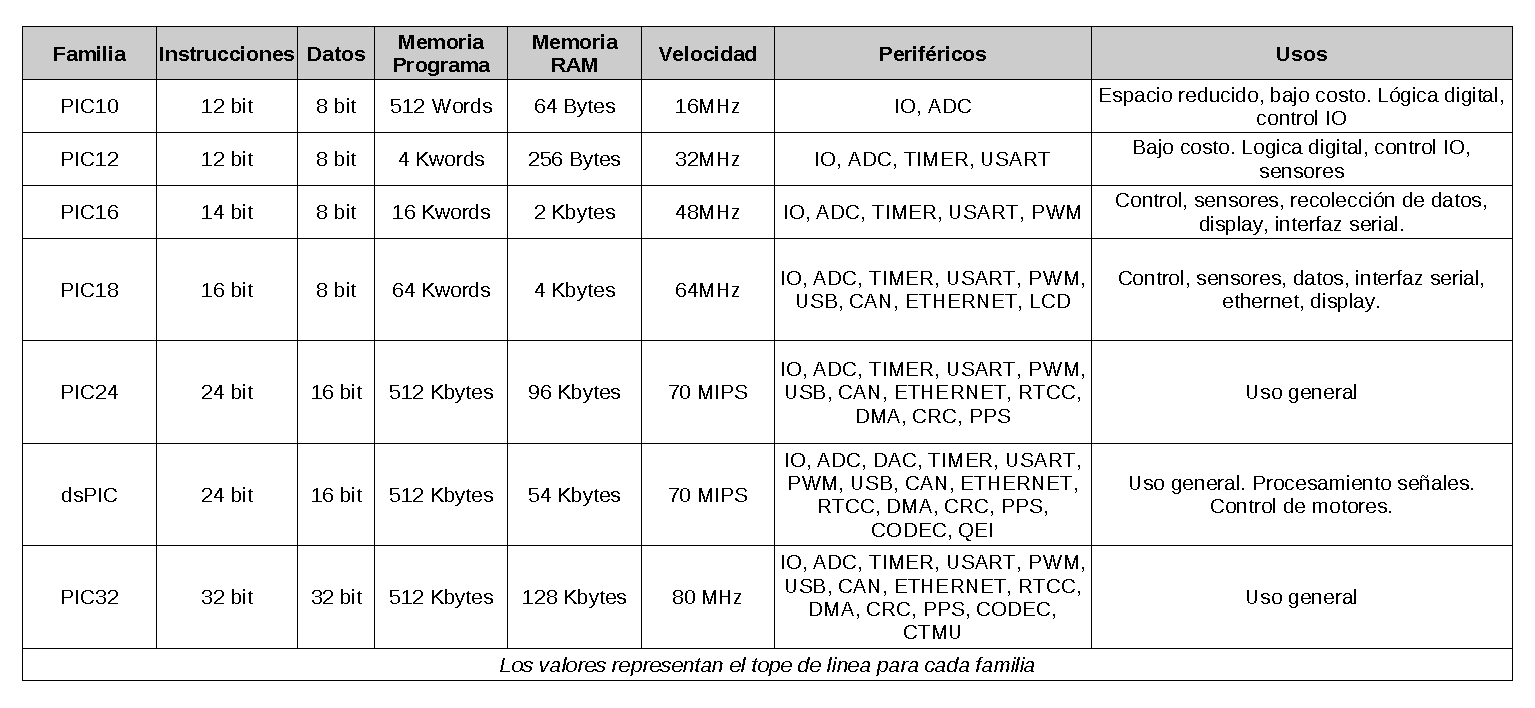
\includegraphics[width=\textwidth]{img/pic_list.pdf}
\end{table}
%··········································

A continuación se describen las características específicas de los microcontroladores PIC24 que corresponde al dispositivo utilizado en este trabajo.

\paragraph{Arquitectura}
Poseen un juego de instrucciones \ac{RISC} (80 instrucciones) de ancho fijo en 24 bits que en su mayoría se ejecutan en un solo ciclo excepto: divisiones; cambios de contexto; y acceso por tabla a memoria de programa\cite{PIC24_PROG}. Se basa en una arquitectura Harvard modificada de 16 bits de datos\cite{PIC24F} lo que significa que el dispositivo posee una memoria de datos tipo \ac{RAM} separada de la memoria de datos (FLASH) pudiendo acceder de manera independiente e incluso simultáneamente a las instrucciones del programa y a los datos de este alojados en \ac{RAM}. La arquitectura de la CPU la completan una \ac{ALU} con \textit{hardware} dedicado para realizar multiplicaciones y divisiones. El detalle de la arquitectura del microcontrolador PIC24 se detalla en la figura \ref{pic_cpu}. También posee un vector de hasta 128 interrupciones con capacidad para atender hasta 8 de ellas lo que permite liberar al procesador de la espera de sucesos asíncronos ya que son notificados y atendidos de manera específica en una rutina de atención de la interrupción.

% ················ IMAGEN ·················
\begin{figure}[ht!]
\centering
\fbox{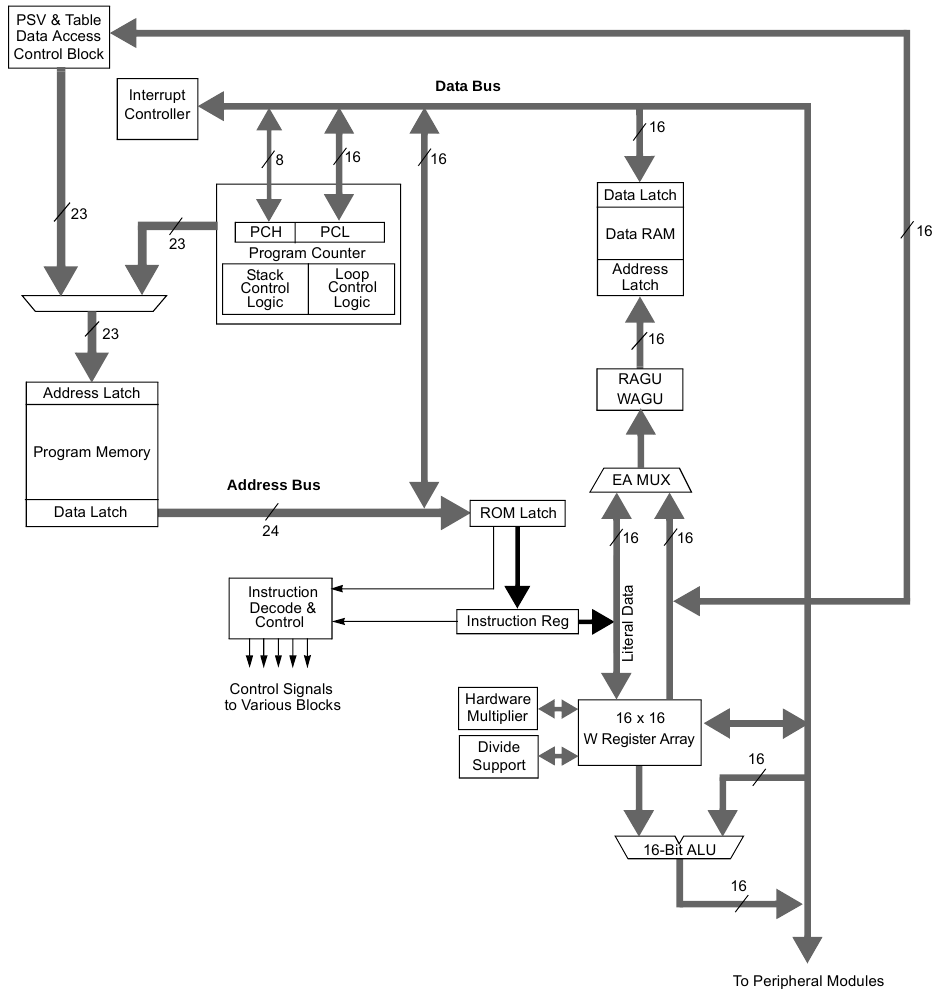
\includegraphics[scale=0.5]{img/pic_cpu.png}}
\caption{Arquitectura de la CPU del PIC24F}\label{pic_cpu}
\end{figure}
%··········································

\paragraph{Periféricos}
La familia de microcontroladores PIC24F integra en el mismo chip una serie de periféricos que permiten realizar funciones específicas a través de hardware especialmente diseñado. Esto hace que el PIC24F se convierta en un sistema embebido capaz de ser utilizados en aplicaciones que requieran: conversores análogos a digitales; temporizadores; comunicación síncronas y asíncronas como RS232, SPI o I2C; USB o Ethernet; manteniendo acotados los costos del sistema. Una lista de los periféricos disponibles para estos microcontroladores se detalla en la figura \ref{pic_perif}. El acceso para configurar, guardar y obtener datos de estos periféricos se realiza a través de registros que están mapeados en la memoria de datos del microcontrolador por lo tanto comparten el bus de datos y no son necesarias instrucciones extras para su integración. Junto con una completa documentación de la arquitectura y funcionamiento de cada periférico, los compiladores de lenguaje C de Microchip proveen librerías para acceder a estas funcionalidades a través de una API de más alto nivel.

% ················ IMAGEN ·················
\begin{figure}[ht!]
\centering
\fbox{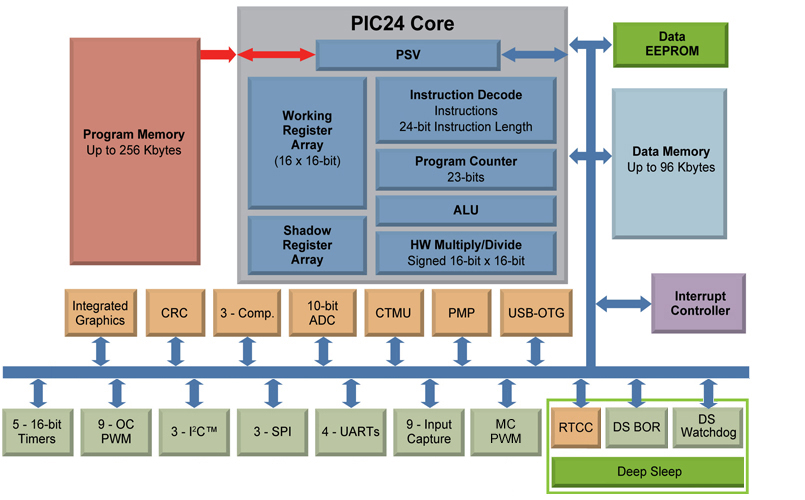
\includegraphics[scale=0.5]{img/pic_perif.jpg}}
\caption{Arquitectura del PIC24F}\label{pic_perif}
\end{figure}
%··········································

% \paragraph{Desarrollo}

% ============= SISTEMAS OPERATIVOS ==============
\subsection{Sistemas Operativos}
Un sistema operativo es la aplicación base de un sistema computacional pues brinda servicios básicos al resto de las aplicaciones de uso general que se ejecutan en el computador. El sistema operativo es la capa entre el hardware y las aplicaciones. El hardware puede variar considerablemente entre un sistema y otro, por eso se necesita una capa de abstracción que haga a la aplicación independiente de la plataforma en que se ejecuta. Para esto el sistema operativo provee servicios que usan interfaces de bajo nivel con el hardware las cuales no están disponibles para la aplicación. La figura \ref{os} es un esquema que ilustra un sistema operativo como una capa de abstracción del hardware. Ejemplos de sistemas operativos los son UNIX, GNU/Linux, FreeRTOS, entre otros.

% ················ IMAGEN ·················
\begin{figure}[ht!]
\centering
\fbox{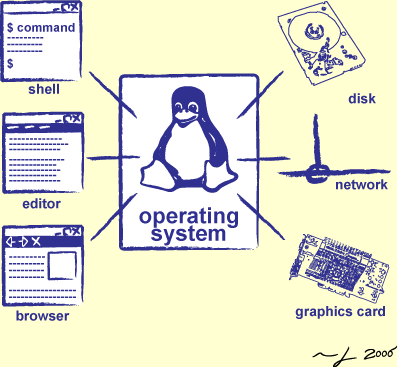
\includegraphics[scale=0.5]{img/os.png}}
\caption{Sistema Operativo como capa de abstracción}\label{os}
\end{figure}
%··········································

\subsubsection{Sistemas Operativos de Tiempo Real}
Parte fundamental de un sistema operativo es su \textit{scheduler}, módulo encargado de intercambiar entre las múltiples tareas que se deben ejecutar cediendo un espacio de tiempo para utilizar le procesador. La forma en que trabaja el \textit{scheduler} define el tipo de sistema operativo que se posee. Un sistema operativo de tiempo real posee un \textit{scheduler} diseñado para proveer un flujo de ejecución determinista, pues solo sabiendo con exactitud la tarea que el sistema ejecutara en un determinado momento se pueden cumplir los requerimientos estrictos de \textit{timing}\cite{FREERTOS}. Esto es un aspecto de especial interés en sistemas embebidos que normalmente requieren respuesta en tiempo real ante eventos no predecibles.\\

La figura \ref{rtos} demuestra la forma de conseguir un sistema de tiempo real mediante el uso de prioridades para las diferentes tareas. En este ejemplo la mayor parte del tiempo el sistema está en estado \textit{idle}, sin código que ejecutar. Sin embargo ante la precencia de ciertos evento el sistema debe responder de manera instantánea cambiado de contexto a la tarea correspondiente. Ciertas tareas pueden requerir un estricto \textit{timing} ejecutándose de manera periódica, por ejemplo. En este caso se asigna una alta prioridad para asegurar que el sistema operativo siempre ejecutara esta tarea cuando corresponda.

% ················ IMAGEN ·················
\begin{figure}[ht!]
\centering
\fbox{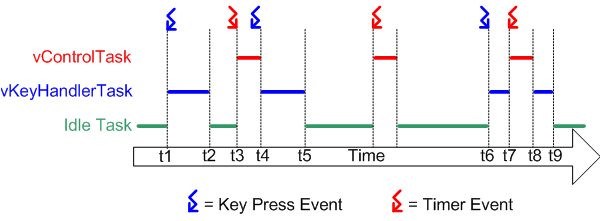
\includegraphics[scale=0.8]{img/rtos.png}}
\caption{\textit{Real time scheduling}}\label{rtos}
\end{figure}
%··········································

\subsubsection{FreeRTOS}
FreeRTOS es un tipo de \ac{RTOS} que está diseñado para ser lo suficientemente pequeño como para ser utilizado en un microcontrolador como sistemas embebidos\cite{FREERTOS}. Como estos sistemas son realmente limitados, normalmente no existe la posibilidad de ejecutar un sistema operativo completo como GNU-Linux, pero FreeRTOS provee un kernel capaz de manejar múltiples tareas con prioridades; comunicación entre tareas; \textit{timing} y primitivas de sincronización. Por su reducido tamaño no provee funcionalidades de alto nivel como una consola de comandos; así como tampoco funcionalidades de bajo nivel como controladores para el hardware o periférico. Entre sus principales características se encuentran:

\begin{itemize}
	\item \textit{Scheduler pre-emptive} o cooperativo.
	\item Sincronización y comunicación entre tareas a través de colas, semáforos, semáforos binarios y mutexes.
	\item Mutexes con herencia de prioridades.
	\item Software \textit{timers}.
	\item Bajo consumo de memoria (Entre 6K y 10K en ROM).
	\item Altamente configurable.
	\item Detección de \textit{stack overflow}
	\item Soporte oficial a 33 arquitecturas de sistemas embebidos.
	\item Estructura de código portable, escrito en C.
	\item Licenciado bajo \ac{GPL} modificada que permite su uso comercial sin publicar código fuente.
	\item Gratuito
	\item Amplia documentación, foros y asistencia técnica.
\end{itemize}

\paragraph{Funcionamiento}
Los conceptos fundamentales detrás del funcionamiento de FreeRTOS son las tareas y el \textit{scheduler}. Una tarea es un hilo de procesamiento, normalmente una función que se ejecuta de manera continua. Una tarea se puede encontrar dos estados fundamentales: ejecutándose y no ejecutándose. Cuando una tarea se está ejecutando tiene el control del procesador y el código dentro de la función que representa a la tarea es procesado. El estado ``no ejecutándose'' en realidad consta de tres sub-estados como se observa en la figura\ref{task_state}: se inicia en un estado ``listo'' lo que indica que la tarea está en condiciones de ser selecciona por el \textit{scheduler} y pasar a estado ``ejecutándose''; el estado ``bloqueado'' significa que la tarea no está disponible para ser ejecutada pues está en espera de algún evento, por ejemplo, la liberación de un mutex; cuando la tarea está en estado ``suspendida'' tampoco se puede ejecutar, la tarea debe explícitamente reanudarse para quedar en condiciones de ser ejecutada.

% ················ IMAGEN ·················
\begin{figure}[ht!]
\centering
\fbox{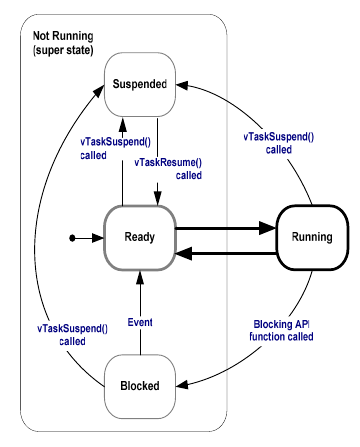
\includegraphics[scale=0.9]{img/task_state.png}}
\caption{Tareas de FreeRTOS, diagrama de estados}\label{task_state}
\end{figure}
%··········································

La creación de taras y el control de sus estados se realiza a través de la API de FreeRTOS que documenta claramente todas las posibles operaciones que se pueden realizar sobre una tarea.\\

El \textit{scheduler} es la parte fundamental del kernel que controla la ejecución de las diferentes tareas disponibles. Su objetivo es generar la sensación de estar en un ambiente multitarea, cuando en realidad sólo una tarea puede ejecutarse a la vez ya que se posee un solo procesador. Como se detalla en la figura \ref{scheduler} la función del \textit{scheduler} es entregar una porción de tiempo de ejecución fijo a una tarea y una vez que este tiempo se cumple se debe guardar el estado de ejecución de esta tarea y se procede a ejecutar otra. Así cada una de las tareas se ejecuta durante una pequeña porción de tiempo, hasta que completa su trabajo; si el tiempo de proceso asignado a cada tarea es lo suficientemente pequeño pareciera que muchas cosas ocurrieron simultáneamente. Claramente una sola tarea tomaría, en términos absolutos, menos tiempo en terminar si no fuera interrumpida, pero se gana un sistema más fluido cuando se deben ejecutar en conjunto tareas que toman mucho tiempo de proceso y otras relativamente cortas.

% ················ IMAGEN ·················
\begin{figure}[ht!]
\centering
\fbox{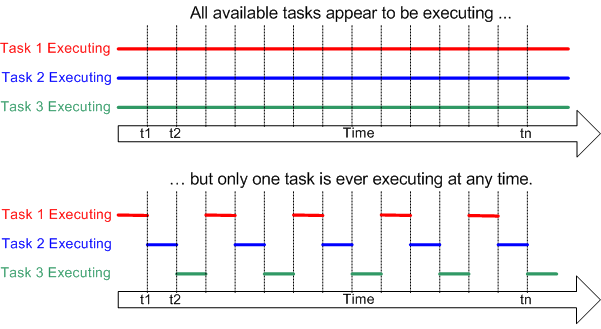
\includegraphics[scale=0.9]{img/scheduler.png}}
\caption{\textit{Scheduling} de tareas}\label{scheduler}
\end{figure}
%··········································

El algoritmo de \textit{scheduling} se basa en un sistema de prioridades, donde la tarea en condiciones de ejecutarse que tenga la mayor prioridad siempre debe ser ejecutada. Si varias tareas en estado ``listo'' comparten la misma prioridad se aplica un algoritmo de \textit{round-robing}. Las tareas que están en estado ``suspendido'' y ``bloqueado'' nunca son seleccionadas por el \textit{scheduler} y por lo tanto no consumen recursos. Haciendo un correcto uso de las prioridades y los diferentes estados se consigue un sistema que se ejecuta de manera fluida y haciendo un uso óptimo del procesador.

% \paragraph{Ejemplo de uso}


% ============= INGENIERIA DE SOFTWARE ==============
\subsection{Ingeniería de Software}

% ============= LICENCIAS DE SOFTWARE ==============
\subsubsection{Licencias de Software}
Se entiende por licencia de software a un contrato entre el desarrollador del software y el usuario final para su utilización según una serie de términos o condiciones. La licencia puede ceder ciertos derechos al usuario final; controlar la cantidad de copias que puede utilizar; el ámbito geográfico y temporal para la utilización; o bien proteger al desarrollador frente a la utilización del programa informático que se licencia. Existen al menos tres tipos de licencias de software:

\begin{itemize}
	\item \textbf{Privativas:}  El software es distribuido al usuario bajo un \ac{EULA} en que el propietario fija las condiciones de uso y se reserva la propiedad del programa informático. Generalmente impide el acceso al código fuente; la realización de ingeniería inversa; el uso del software por más de un usuario; se entrega el derecho de uso por un tiempo definido y por lo general provee cierta asesoría técnica. Es común que se debe pagar por el uso de un programa bajo este tipo de licencia.
	
	\item \textbf{Libres:} Este tipo de licencias otorgan al receptor la libertad de usar, estudiar, compartir y modificar el software. Existen varias licencias que cumplen con esta definición, por ejeplo: MIT, BSD, \ac{LGPL} y \ac{GPL}. Se dividen en dos tipos básicos licencias con \textit{copyleft} y sin \textit{copyleft}. Se habla de una licencia con \textit{copyleft} cuando esta indica que el software derivado debe mantener la misma licencia original impidiendo la generación de software privativo a partir de desarrollos libres, por ejemplo. Por lo general cumplir esta licencia requiere que se garantice el acceso al código fuente, de aquí el termino conocido como software de código abierto. La mayoría del software bajo estas licencias se distribuye de forma gratuita aunque su uso comercial no está necesariamente prohibido. No todo software gratuito es necesariamente software libre.
	
	\item \textbf{Dominio Público:} Si un programa informático se distribuye sin ningún tipo de licencia, se dice que es de dominio público. No posee ningún tipo de restricción sobre su uso, así como ninguna responsabilidad sobre sus creadores.
\end{itemize}

La aplicación de licencias se rige según las normativas legales locales. En el caso de las licencias libres por lo general basta con distribuir el texto de la licencia junto con la aplicación y agregar un encabezado indicando el tipo de licencia que se utiliza. Para atribuir autoría se suele utilizar las definiciones de la Convención de Berna, que indica que todo lo que se escribe queda automáticamente sujeto a copyright desde el momento en que la obra es fijada en un soporte material\cite{GNU}. En Chile la legislación vigente al respecto es la Ley 17.336 de propiedad Intelectual.

\subsubsection{\ac{GPL}}
La \ac{GPL} es una licencia de software creada en 1989 por la \textit{Free Software Foundation} que busca declarar que el software así licenciado es software libre y por lo tanto el usuario posee los siguientes derechos\cite{GPL}:
\begin{itemize}
	\item Libertad de usar el software para cualquier propósito.
	\item Libertad de modificar el software para adaptarlo a las propias necesidades.
	\item Libertad para compartir el software.
	\item Libertad para publicar los cambios que se han realizado.
\end{itemize}

Actualmente se encuentra en su versión 3.0 que a diferencia de versiones previas es una licencia con \textit{copyleft} y agrega cláusulas para proteger la libertad del usuario frente a nuevas prácticas en contra del software libre, tales como\cite{GPL}:
\begin{itemize}
	\item Tivoización: El término se refiere a la práctica de limitar los derechos de los usuarios que compran sistemas que funcionan con software libre mediante mecanismos de hardware, por ejemplo evitando la ejecución de versiones modificadas del software embebido.
	\item Leyes que prohíben software libre: Se asegura de que ciertas leyes puedan limitar los derechos del usuario de un software con licencia \ac{GPL}.
	\item Uso malicioso de patentes: Evita el uso indiscriminado de patentes, como por ejemplo, intentar obtener beneficios patentado desarrollos de software libre lo cual es una amenaza a la liberta de los usuarios.
\end{itemize}

\paragraph{Aplicación de la licencia} Para licenciar un proyecto de software libre bajo la \ac{GPL} V3.0 se deben seguir los siguientes pasos\cite{GNU}:
\begin{enumerate}
	\item Agregar un aviso informativo del \textit{copyright} al inicio de cada archivo con código fuente de la aplicación. Un ejemplo es la siguiente línea: \texttt{«Copyright 2012 Universidad de Chile»}
	
	\item Bajo el aviso de \textit{copyright} se agrega una autorización de copia indicando que el software se distribuye bajo los términos de la licencia \ac{GPL}. Un ejemplo de este aviso se cita en un ejemplo posterior.
	
	\item Se debe incluir junto al código fuente el texto completo de la licencia en un archivo llamado \texttt{LICENSE}. El texto de la licencia se puede obtener desde el siguiente enlace: \url{http://www.gnu.org/licenses/gpl.txt}.
\end{enumerate}

A continuación se detalla el encabezado que debería incluir cada fichero del proyecto de software hipotético llamado \texttt{Foobar}  que es licenciado bajo \ac{GPL}.

\begin{verbatim}
    Foobar - Description - «Copyright 2012 Universidad de Chile»
	
    This file is part of Foobar.

    Foobar is free software: you can redistribute it and/or modify
    it under the terms of the GNU General Public License as published by
    the Free Software Foundation, either version 3 of the License, or
    (at your option) any later version.

    Foobar is distributed in the hope that it will be useful,
    but WITHOUT ANY WARRANTY; without even the implied warranty of
    MERCHANTABILITY or FITNESS FOR A PARTICULAR PURPOSE.  See the
    GNU General Public License for more details.

    You should have received a copy of the GNU General Public License
    along with Foobar.  If not, see <http://www.gnu.org/licenses/>.
\end{verbatim}




% ============= BIBLIOGRAFIA ==============
\newpage
\begin{thebibliography}{50}
% Manuales
	\bibitem{MPLAB} Microchip, \textit{MPLABX IDE User's Guide}, USA:  Microchip Technology Incorporated, 2011.
	\bibitem{PIC24F} Microchip, \textit{PIC24F Family Reference Manual}, USA:  Microchip Technology Incorporated, 2006.
	\bibitem{PIC24_PROG} Microchip, \textit{16 bit MCU and DSC Programmer's Reference Manual}, USA:  Microchip Technology Incorporated, 2011.
	\bibitem{PIC24FJ256GA110} Microchip, \textit{PIC24FJ256GA110 Datasheet}, USA:  Microchip Technology Incorporated, 2006.
	\bibitem{FREERTOS_PIC24} R. Barry, \textit{Using the FreeRTOS Real Time Kernel. A Practical Guide, PIC32 Edition.}, 1st ed., USA: Real Time Engineers, 2009.
	\bibitem{FREERTOS_API} R. Barry, \textit{The FreeRTOS Reference Manual}, 1st ed., USA: Real Time Engineers, 2011.

% Libros
	\bibitem{SE} I. Sommerville, \textit{Software Engineering}, 9nd ed., USA: Addison-Wesley, 2011.
	\bibitem{EMBEDDED} S. Heat, \textit{Embedded Systems Design}, 2nd ed., England: Newnes, 2003.
	\bibitem{FLYPIC} L. Di Jasio \textit{Programming 16-Bit PIC Microcontrollers in C} , 1st ed. USA: Elsevier, 2007.
	
% Recursos Web
%Directorio de servicios de préstamo interbibliotecario de Rebiun [en línea]. Barcelona: Universitat Pompeu Fabra, 1996- . "Universidad Nacional de Educación a Distancia". <http://www.upf.es/bib/pinter/uned.htm> [Consulta: 6 mayo 1997].
	\bibitem{GPL} Free Software Foundation. \textit{GNU General Public License} [En Línea]. USA, 2011. \url{http://www.gnu.org/licenses/gpl.html} [Consulta: 22 noviembre 2012]
	\bibitem{GNU} Free Software Foundation. \textit{Preguntas frecuentes acerca de las licencias de GNU} [En Línea]. USA, 2011. \url{http://www.gnu.org/licenses/gpl-faq.html} [Consulta: 22 noviembre 2012]
	\bibitem{FREERTOS} Real Time Engineers. \textit{About FreeRTOS} [En Línea]. USA, 2012. \url{http://www.freertos.org/about-RTOS.html} [Consulta: 22 noviembre 2012]
	
\end{thebibliography}

\end{document}

% % ················ IMAGEN ·················
% \begin{figure}[ht!]
% \centering
% \fbox{\includegraphics[scale=0.6]{img/flujo.png}}
% \caption{Flujo de caja anual}\label{flujo}
% \end{figure}
% %··········································

% % ················ IMAGEN ·················
% \begin{figure}[ht!] \centering
% \subfloat[Esquemático]{\includegraphics[scale=0.44]{img/seguidor.png}}
% \subfloat[Simulación]{\includegraphics[scale=0.45]{img/seguidor1.png}}
% \caption{Simulación como seguidor de voltaje}\label{seguidor}
% \end{figure}
% %··········································

% % ················ TALBA ·················
% \begin{table}[ht!]
% \caption{Tabla}\label{Tabla}
% \centering \includegraphics[width=\textwidth]{img/flujo.png}
% \end{table}
% %··········································